\documentclass{article}\usepackage[]{graphicx}\usepackage[]{color}
%% maxwidth is the original width if it is less than linewidth
%% otherwise use linewidth (to make sure the graphics do not exceed the margin)
\makeatletter
\def\maxwidth{ %
  \ifdim\Gin@nat@width>\linewidth
    \linewidth
  \else
    \Gin@nat@width
  \fi
}
\makeatother

\definecolor{fgcolor}{rgb}{0.345, 0.345, 0.345}
\newcommand{\hlnum}[1]{\textcolor[rgb]{0.686,0.059,0.569}{#1}}%
\newcommand{\hlstr}[1]{\textcolor[rgb]{0.192,0.494,0.8}{#1}}%
\newcommand{\hlcom}[1]{\textcolor[rgb]{0.678,0.584,0.686}{\textit{#1}}}%
\newcommand{\hlopt}[1]{\textcolor[rgb]{0,0,0}{#1}}%
\newcommand{\hlstd}[1]{\textcolor[rgb]{0.345,0.345,0.345}{#1}}%
\newcommand{\hlkwa}[1]{\textcolor[rgb]{0.161,0.373,0.58}{\textbf{#1}}}%
\newcommand{\hlkwb}[1]{\textcolor[rgb]{0.69,0.353,0.396}{#1}}%
\newcommand{\hlkwc}[1]{\textcolor[rgb]{0.333,0.667,0.333}{#1}}%
\newcommand{\hlkwd}[1]{\textcolor[rgb]{0.737,0.353,0.396}{\textbf{#1}}}%
\let\hlipl\hlkwb

\usepackage{framed}
\makeatletter
\newenvironment{kframe}{%
 \def\at@end@of@kframe{}%
 \ifinner\ifhmode%
  \def\at@end@of@kframe{\end{minipage}}%
  \begin{minipage}{\columnwidth}%
 \fi\fi%
 \def\FrameCommand##1{\hskip\@totalleftmargin \hskip-\fboxsep
 \colorbox{shadecolor}{##1}\hskip-\fboxsep
     % There is no \\@totalrightmargin, so:
     \hskip-\linewidth \hskip-\@totalleftmargin \hskip\columnwidth}%
 \MakeFramed {\advance\hsize-\width
   \@totalleftmargin\z@ \linewidth\hsize
   \@setminipage}}%
 {\par\unskip\endMakeFramed%
 \at@end@of@kframe}
\makeatother

\definecolor{shadecolor}{rgb}{.97, .97, .97}
\definecolor{messagecolor}{rgb}{0, 0, 0}
\definecolor{warningcolor}{rgb}{1, 0, 1}
\definecolor{errorcolor}{rgb}{1, 0, 0}
\newenvironment{knitrout}{}{} % an empty environment to be redefined in TeX

\usepackage{alltt}
\usepackage[utf8]{inputenc}
\usepackage{hyperref}
\hypersetup{
    linktocpage,
    colorlinks=true, 
    linkcolor=blue,
    citecolor=blue,
    filecolor=blue,
    urlcolor=blue
}
\IfFileExists{upquote.sty}{\usepackage{upquote}}{}
\begin{document}

\title{Transcription vs Metilation}
\author{Lucas Michel Todó}
\maketitle
\tableofcontents
\clearpage





\section{Taules Resum}
\subsection{Regió 5'}
\begin{knitrout}
\definecolor{shadecolor}{rgb}{0.969, 0.969, 0.969}\color{fgcolor}\begin{kframe}
\begin{verbatim}
## [1] "10G"
##    Min. 1st Qu.  Median    Mean 3rd Qu.    Max. 
##   0.000   6.168  20.625  23.257  39.611  73.439 
## [1] "1.2B"
##    Min. 1st Qu.  Median    Mean 3rd Qu.    Max. 
##  0.1658  8.7016 22.4585 24.6031 40.7734 77.9003 
## [1] "A7"
##    Min. 1st Qu.  Median    Mean 3rd Qu.    Max. 
##  0.0329  3.9318 11.4498 16.0599 27.7855 58.0386 
## [1] "C2"
##    Min. 1st Qu.  Median    Mean 3rd Qu.    Max. 
##   0.000   2.665   8.495   9.504  15.241  31.232 
## [1] "E5"
##    Min. 1st Qu.  Median    Mean 3rd Qu.    Max. 
##   0.000   2.223   7.263  11.783  20.321  51.756
\end{verbatim}
\end{kframe}
\end{knitrout}
\subsection{ORF}
\begin{knitrout}
\definecolor{shadecolor}{rgb}{0.969, 0.969, 0.969}\color{fgcolor}\begin{kframe}
\begin{verbatim}
##    Min. 1st Qu.  Median    Mean 3rd Qu.    Max. 
##   10.31   66.11   79.51   78.46   92.62  132.52 
##    Min. 1st Qu.  Median    Mean 3rd Qu.    Max. 
##   11.60   67.29   80.06   78.89   92.90  127.29 
##    Min. 1st Qu.  Median    Mean 3rd Qu.    Max. 
##   10.13   49.79   61.61   59.44   71.20   93.74 
##    Min. 1st Qu.  Median    Mean 3rd Qu.    Max. 
##   4.831  32.648  38.811  46.081  53.802 114.518 
##    Min. 1st Qu.  Median    Mean 3rd Qu.    Max. 
##   8.573  39.413  55.289  51.499  63.227  91.169
\end{verbatim}
\end{kframe}
\end{knitrout}
\subsection{Regió 3'}
\begin{knitrout}
\definecolor{shadecolor}{rgb}{0.969, 0.969, 0.969}\color{fgcolor}\begin{kframe}
\begin{verbatim}
##    Min. 1st Qu.  Median    Mean 3rd Qu.    Max. 
##   1.446   3.277   7.517   8.401  10.987  40.575 
##    Min. 1st Qu.  Median    Mean 3rd Qu.    Max. 
##   1.740   3.978  11.271  11.563  16.367  42.265 
##    Min. 1st Qu.  Median    Mean 3rd Qu.    Max. 
##   1.448   3.323   5.297   6.251   8.719  22.439 
##    Min. 1st Qu.  Median    Mean 3rd Qu.    Max. 
##   1.166   2.332   4.081   4.512   6.080  17.490 
##    Min. 1st Qu.  Median    Mean 3rd Qu.    Max. 
##  0.6747  1.4685  2.1830  2.5578  3.3340  9.4463
\end{verbatim}
\end{kframe}
\end{knitrout}
\clearpage


\section{Gràfics}
\subsection{Coverage}
\begin{knitrout}
\definecolor{shadecolor}{rgb}{0.969, 0.969, 0.969}\color{fgcolor}
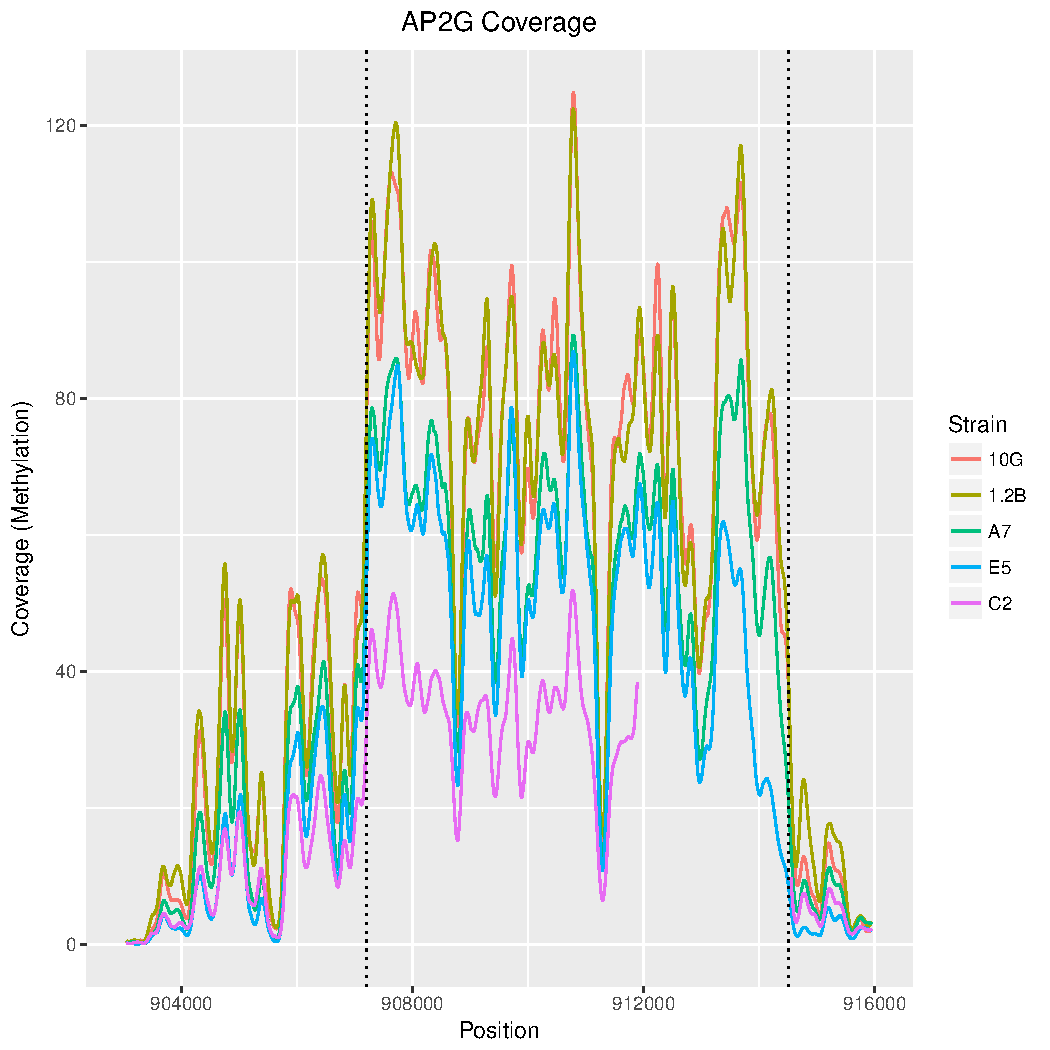
\includegraphics[width=1\linewidth]{figure/plot_coverage-1} 

\end{knitrout}
\clearpage
\subsection{Coverage Normalitzat}
\begin{knitrout}
\definecolor{shadecolor}{rgb}{0.969, 0.969, 0.969}\color{fgcolor}
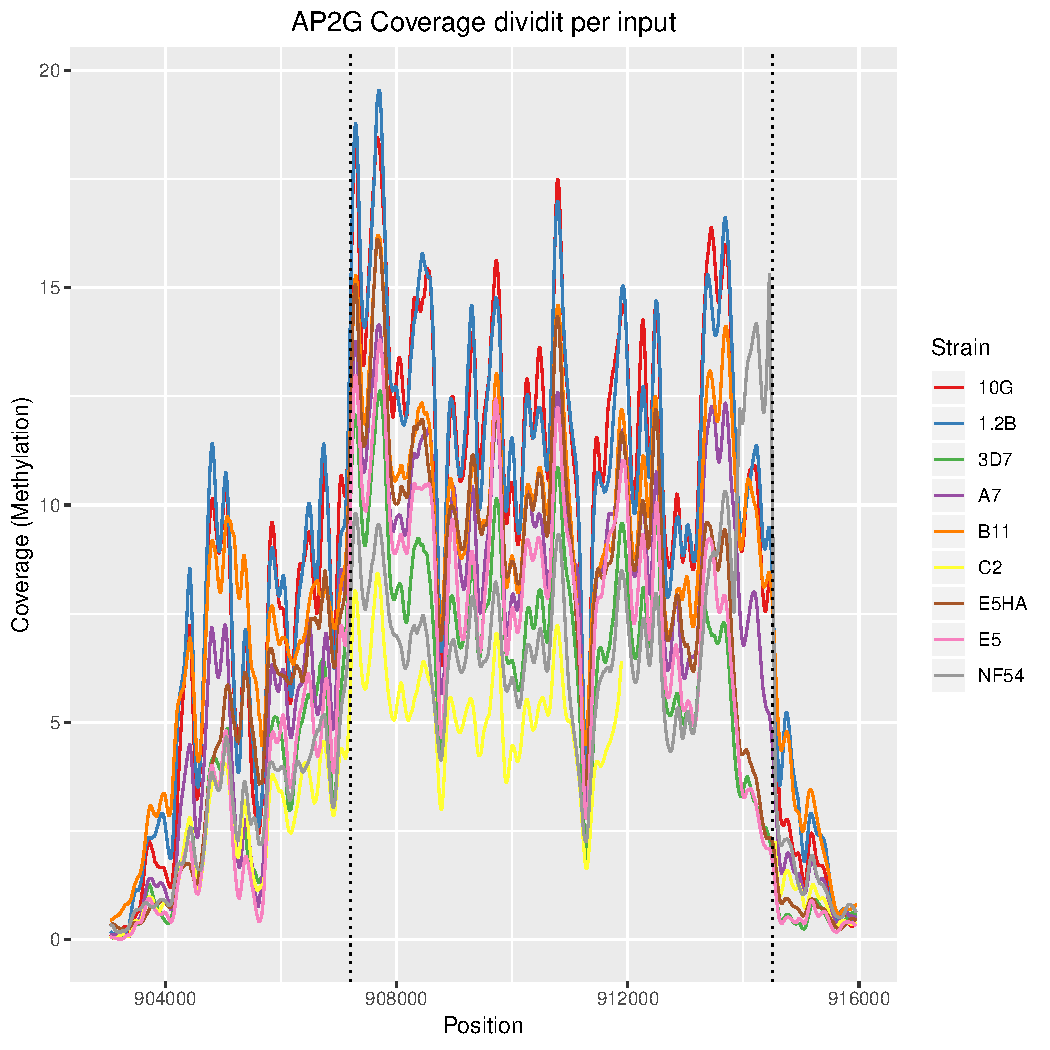
\includegraphics[width=1\linewidth]{figure/plot_norm_cov-1} 

\end{knitrout}
\clearpage
\subsection{Coverage "Equalitzat"}
\begin{knitrout}
\definecolor{shadecolor}{rgb}{0.969, 0.969, 0.969}\color{fgcolor}
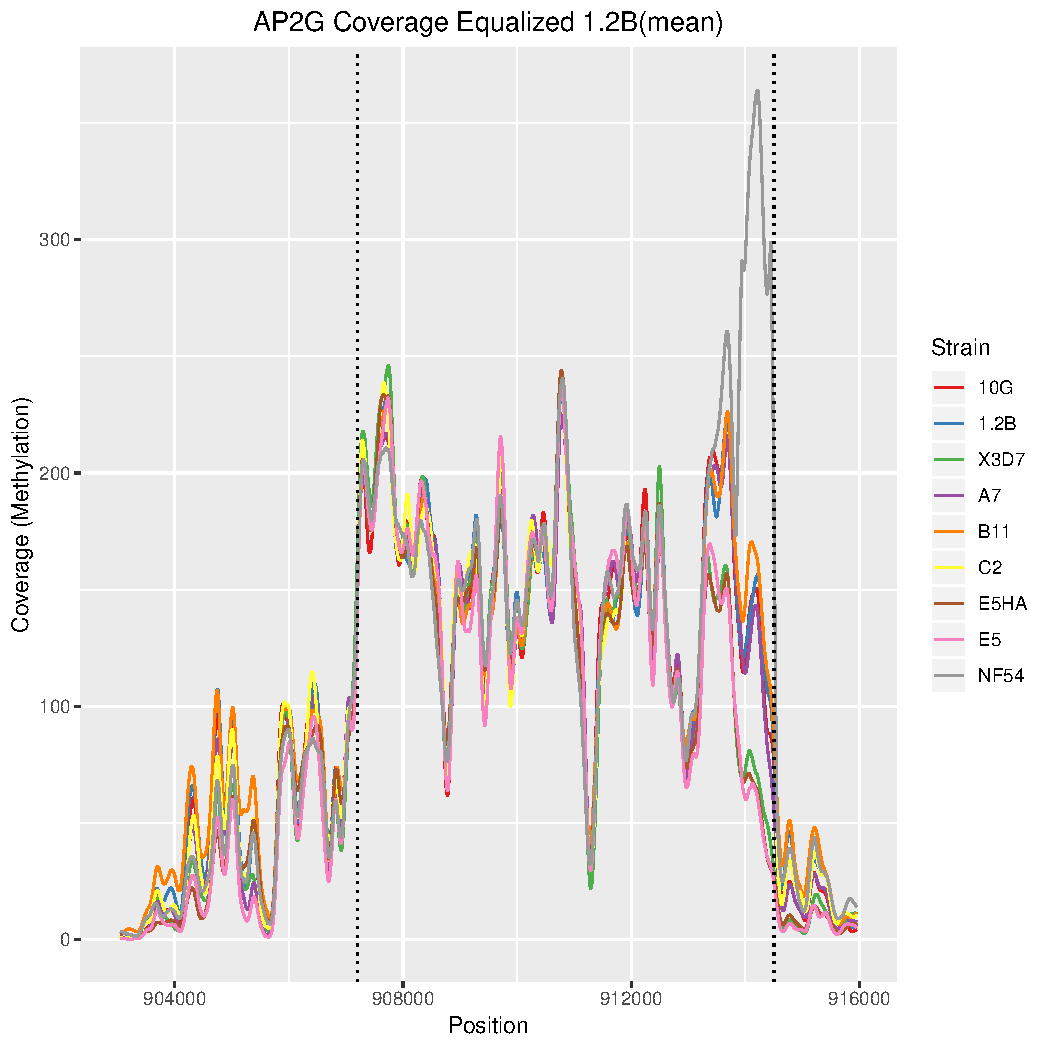
\includegraphics[width=1\linewidth]{figure/plot_equalizedCov-1} 

\end{knitrout}
\clearpage
\subsection{Coverage "Equalitzat": 10G vs 1.2B}
\begin{knitrout}
\definecolor{shadecolor}{rgb}{0.969, 0.969, 0.969}\color{fgcolor}
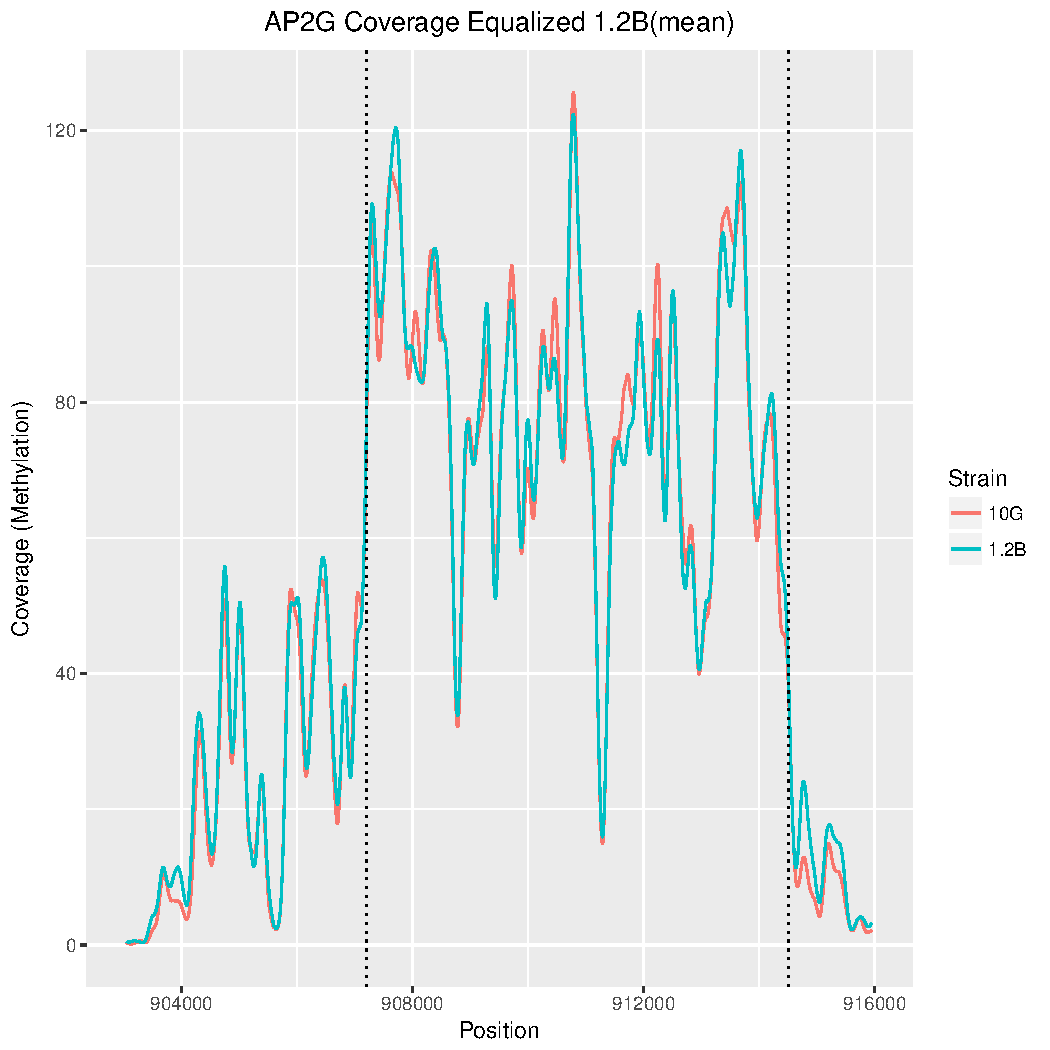
\includegraphics[width=1\linewidth]{figure/plot_equalizedCov_10vs1_2-1} 

\end{knitrout}
\clearpage
\subsection{Coverage "Equalitzat": 10G, E5, A7}
\begin{knitrout}
\definecolor{shadecolor}{rgb}{0.969, 0.969, 0.969}\color{fgcolor}
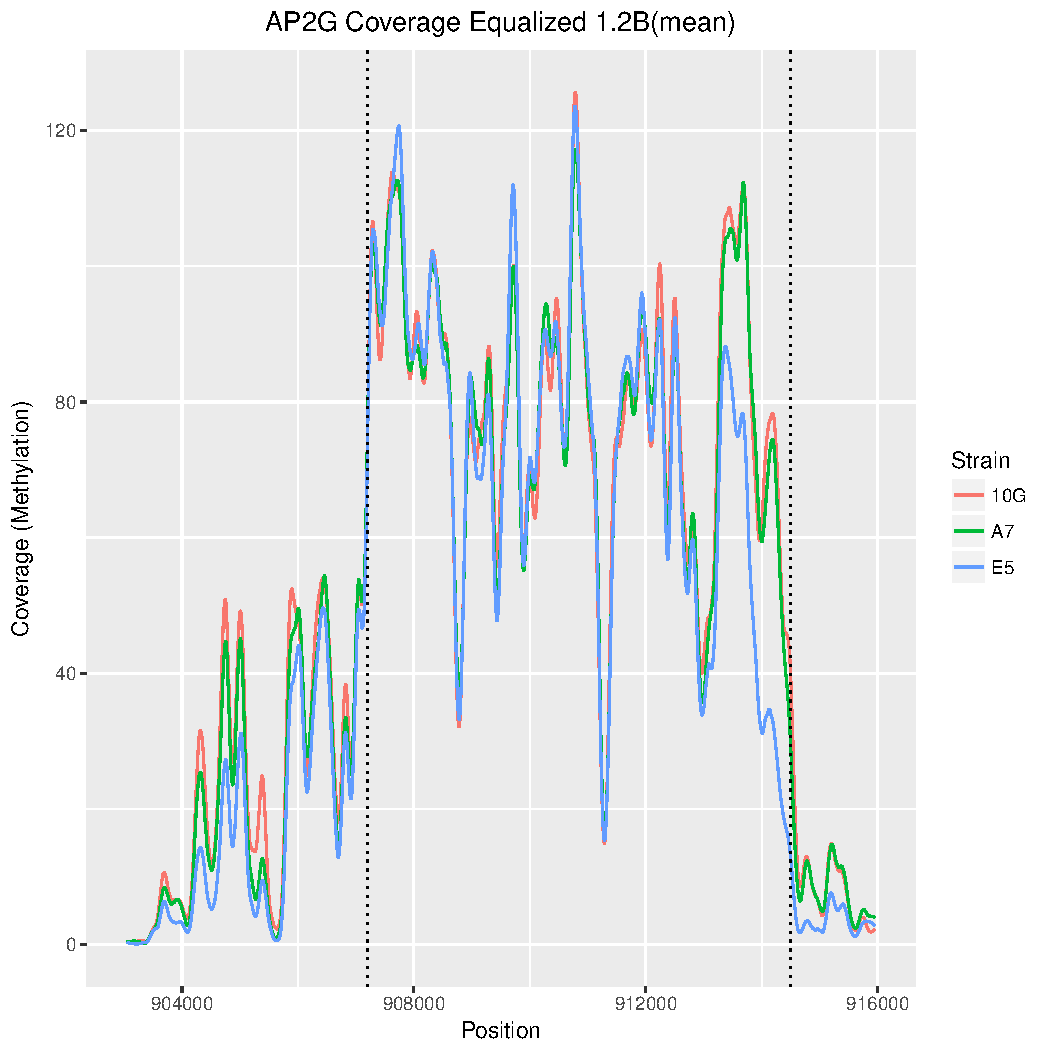
\includegraphics[width=1\linewidth]{figure/plot_equalizedCov_3sample-1} 

\end{knitrout}
\clearpage
\subsection{Coverage Normalitzat i "Equalitzat"}
\begin{knitrout}
\definecolor{shadecolor}{rgb}{0.969, 0.969, 0.969}\color{fgcolor}
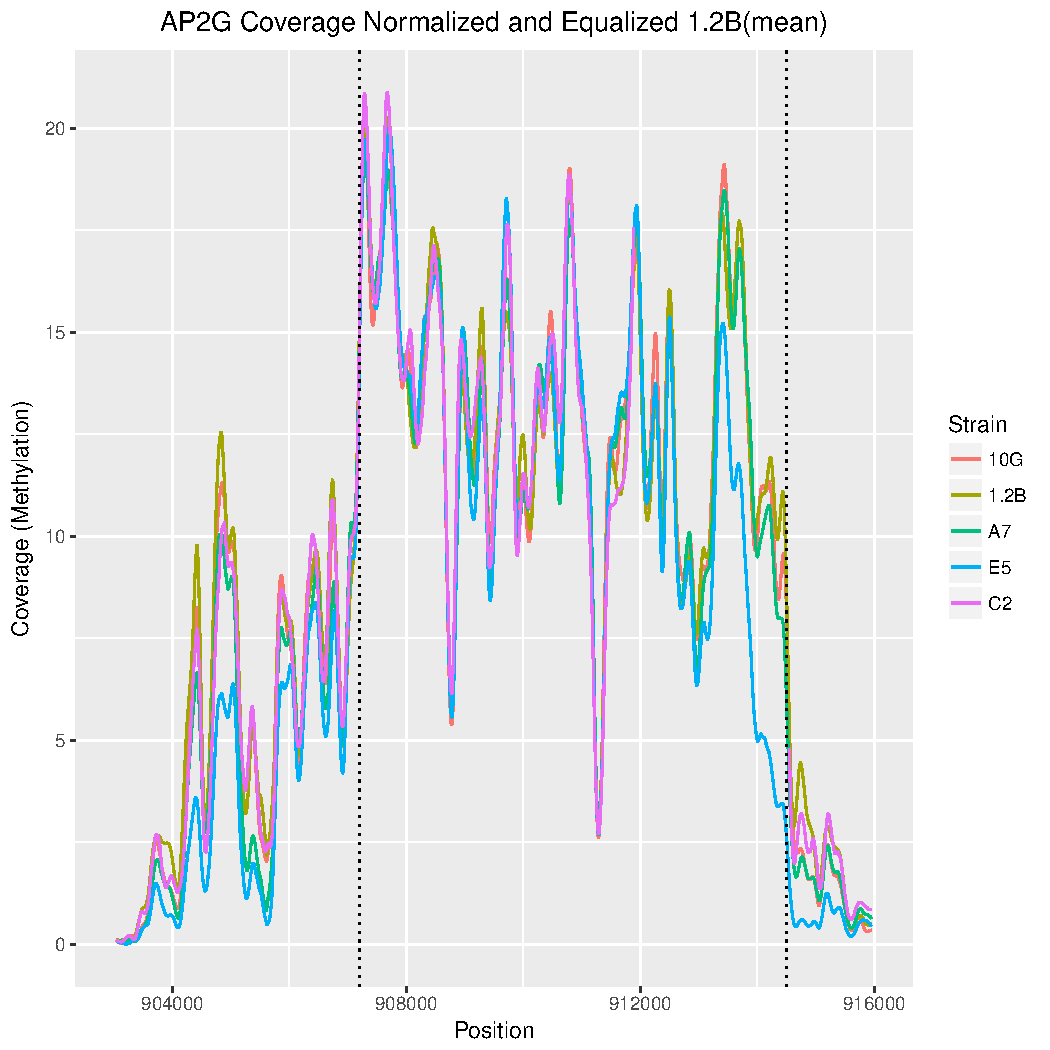
\includegraphics[width=1\linewidth]{figure/plot_NormequalizedCov-1} 

\end{knitrout}
\clearpage
\subsection{Coverage Normalitzat i "Equalitzat": 10G, 1.2B}
\begin{knitrout}
\definecolor{shadecolor}{rgb}{0.969, 0.969, 0.969}\color{fgcolor}
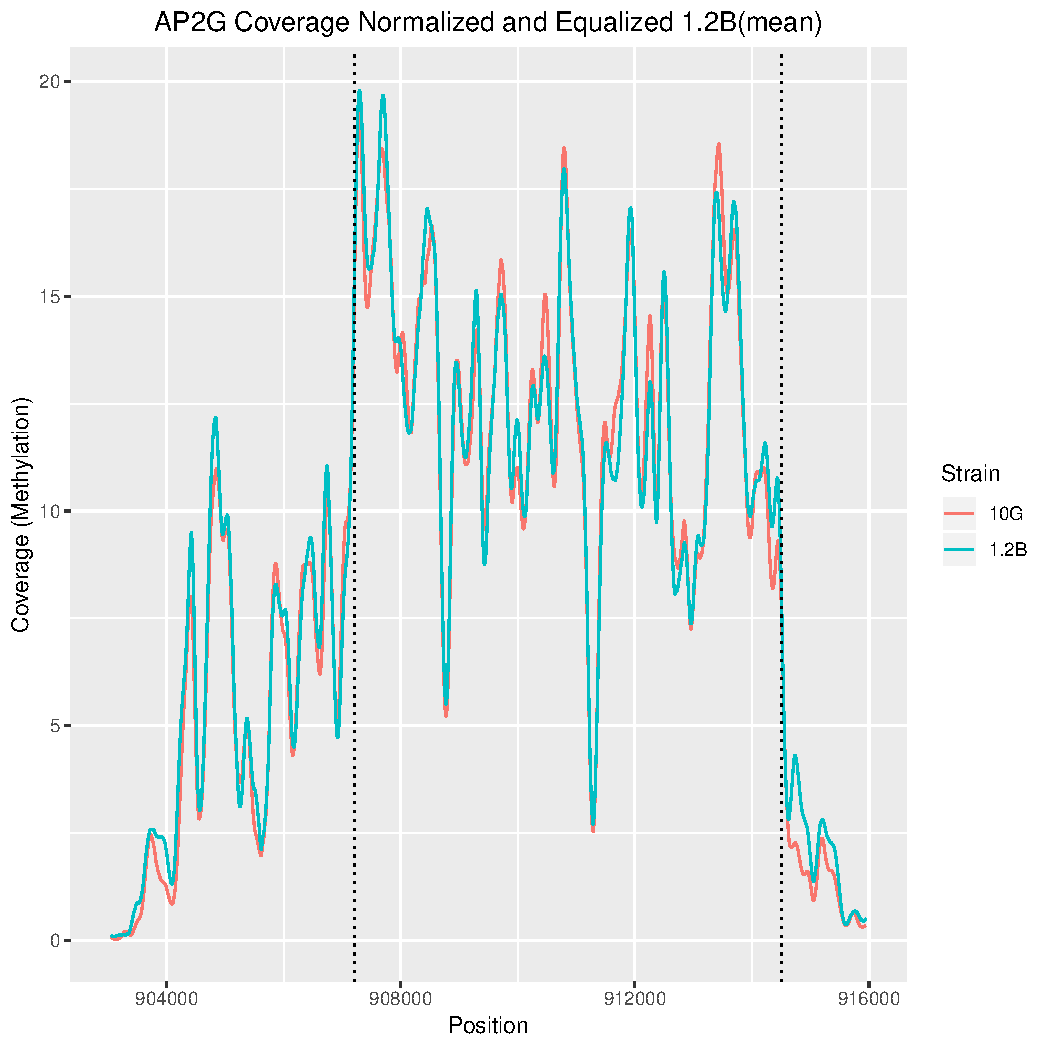
\includegraphics[width=1\linewidth]{figure/plot_NromequalizedCov_10vs1_2-1} 

\end{knitrout}
\clearpage
\subsection{Coverage Normalitzat i "Equalitzat": 10G, E5, A7}
\begin{knitrout}
\definecolor{shadecolor}{rgb}{0.969, 0.969, 0.969}\color{fgcolor}
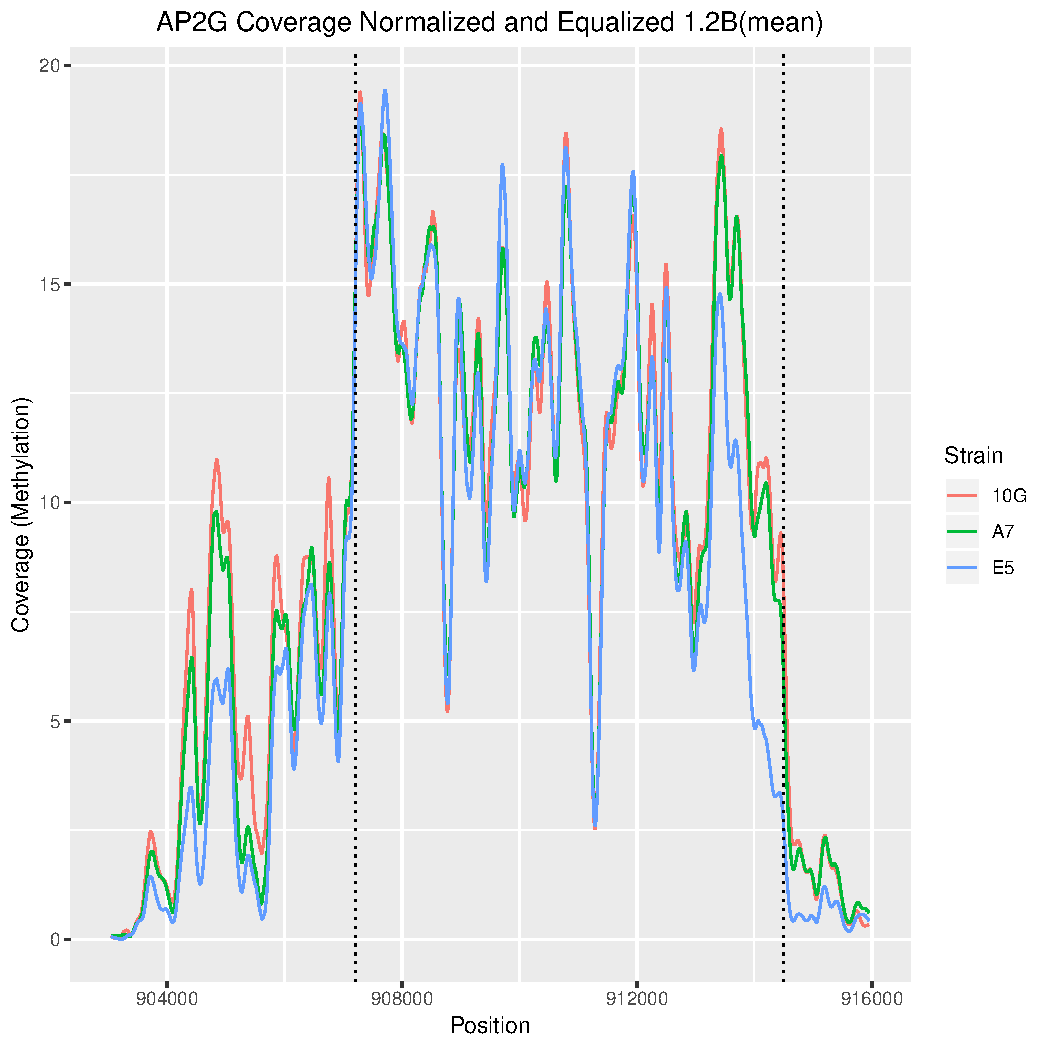
\includegraphics[width=1\linewidth]{figure/plot_NromequalizedCov_3sample-1} 

\end{knitrout}
\clearpage
\subsection{Coverage Normalitzat a regió 5'}
\begin{knitrout}
\definecolor{shadecolor}{rgb}{0.969, 0.969, 0.969}\color{fgcolor}
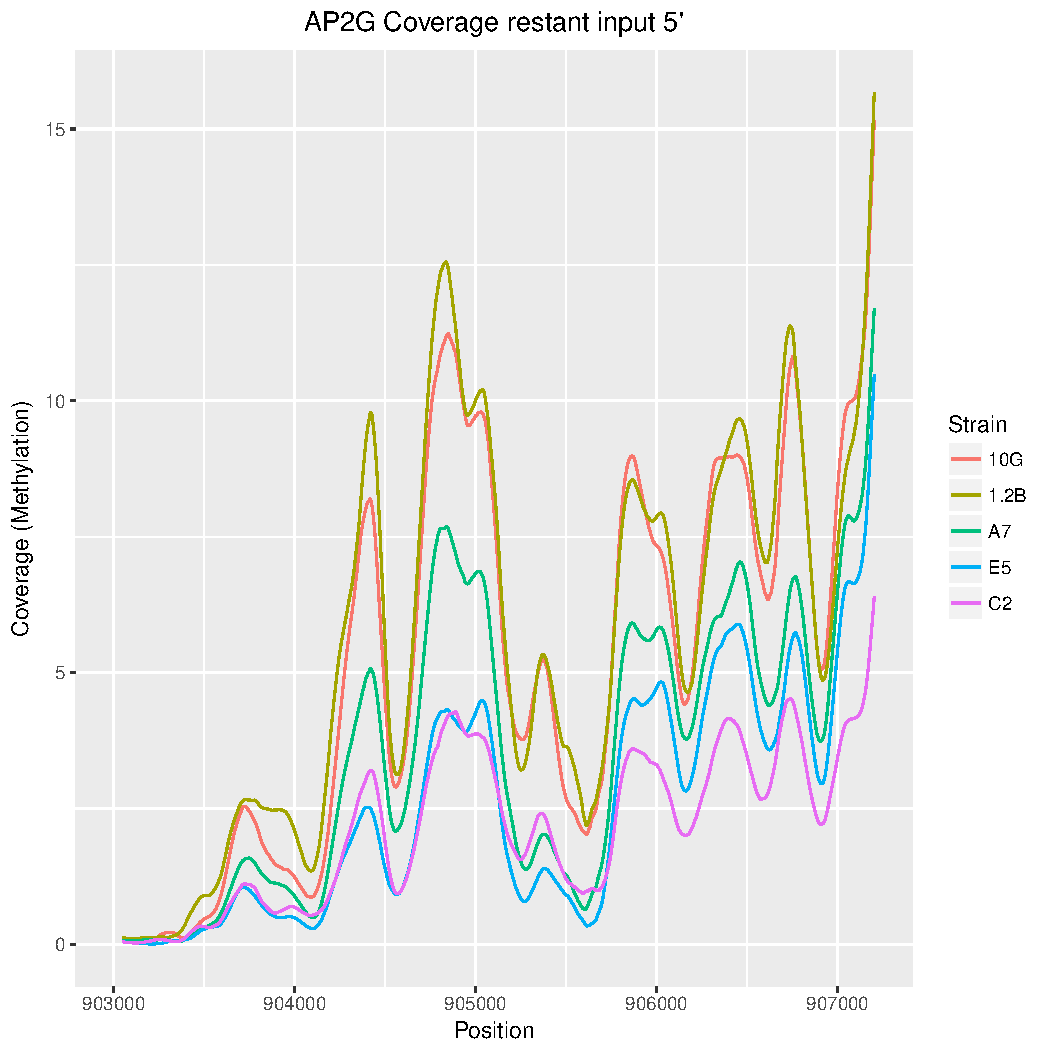
\includegraphics[width=1\linewidth]{figure/plot_norm_cov_5-1} 

\end{knitrout}
\clearpage
\subsection{Coverage Acetilació}
\begin{knitrout}
\definecolor{shadecolor}{rgb}{0.969, 0.969, 0.969}\color{fgcolor}
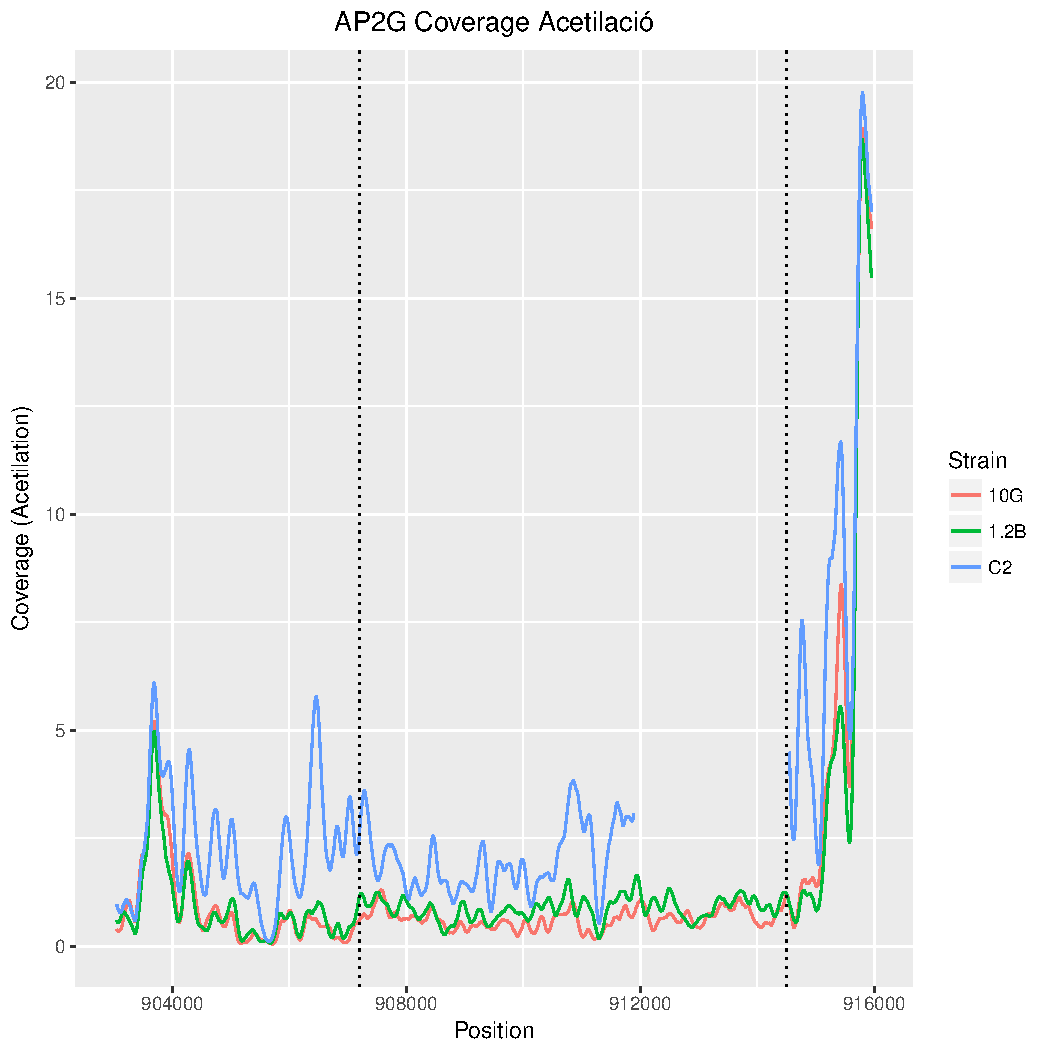
\includegraphics[width=1\linewidth]{figure/plot_ac-1} 

\end{knitrout}
\clearpage
\subsection{Coverage Acetilació a 5'}
\begin{knitrout}
\definecolor{shadecolor}{rgb}{0.969, 0.969, 0.969}\color{fgcolor}
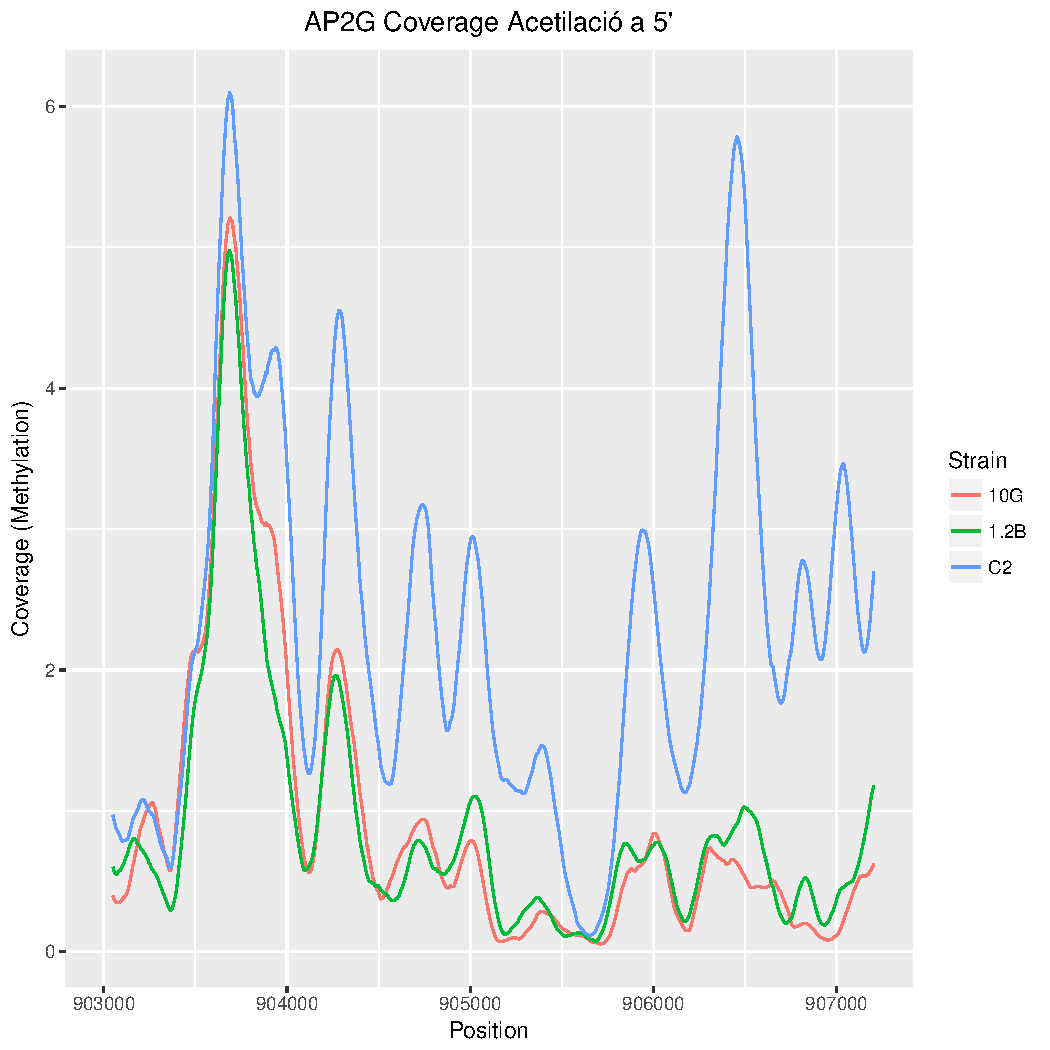
\includegraphics[width=1\linewidth]{figure/plot_ac_5-1} 

\end{knitrout}
\clearpage
\begin{knitrout}
\definecolor{shadecolor}{rgb}{0.969, 0.969, 0.969}\color{fgcolor}
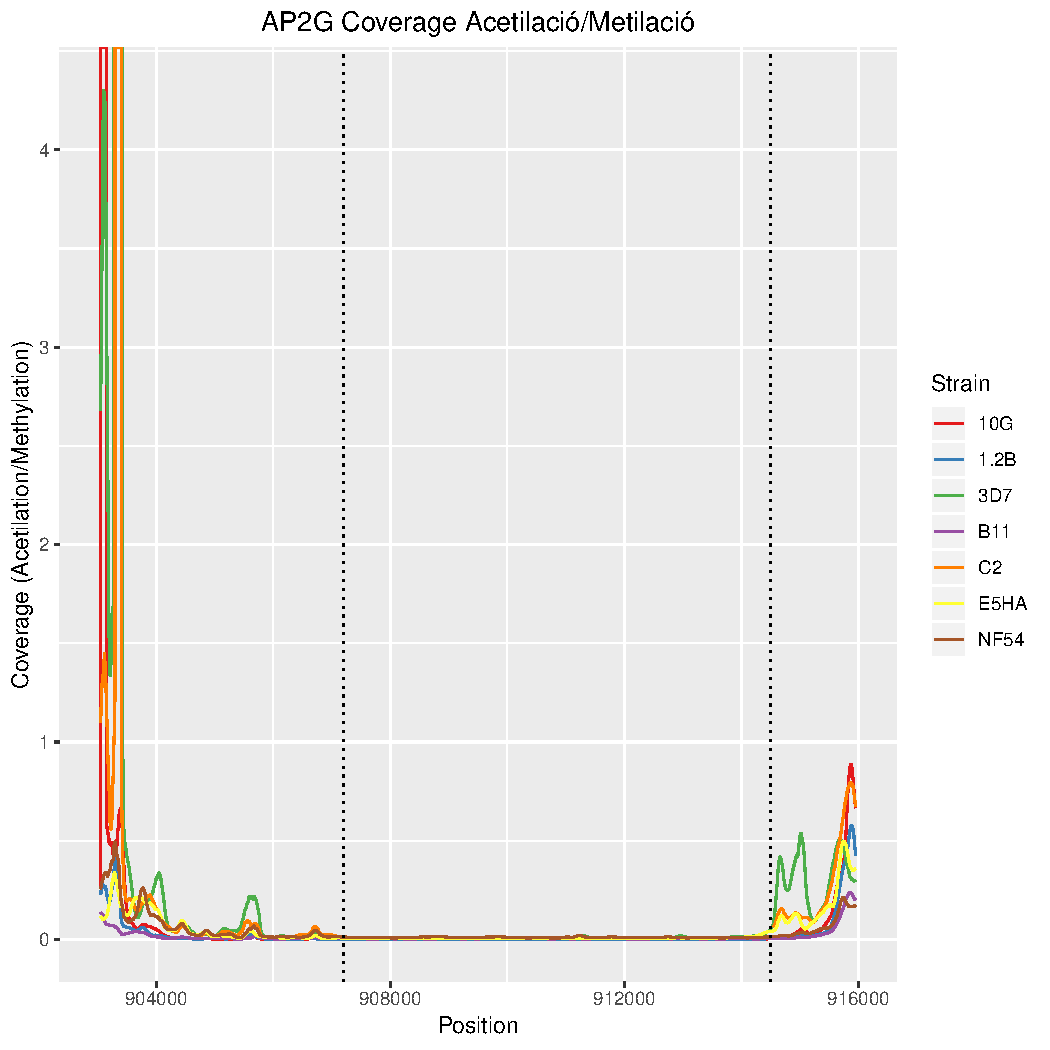
\includegraphics[width=1\linewidth]{figure/Ac_Met-1} 

\end{knitrout}
\clearpage
\begin{knitrout}
\definecolor{shadecolor}{rgb}{0.969, 0.969, 0.969}\color{fgcolor}
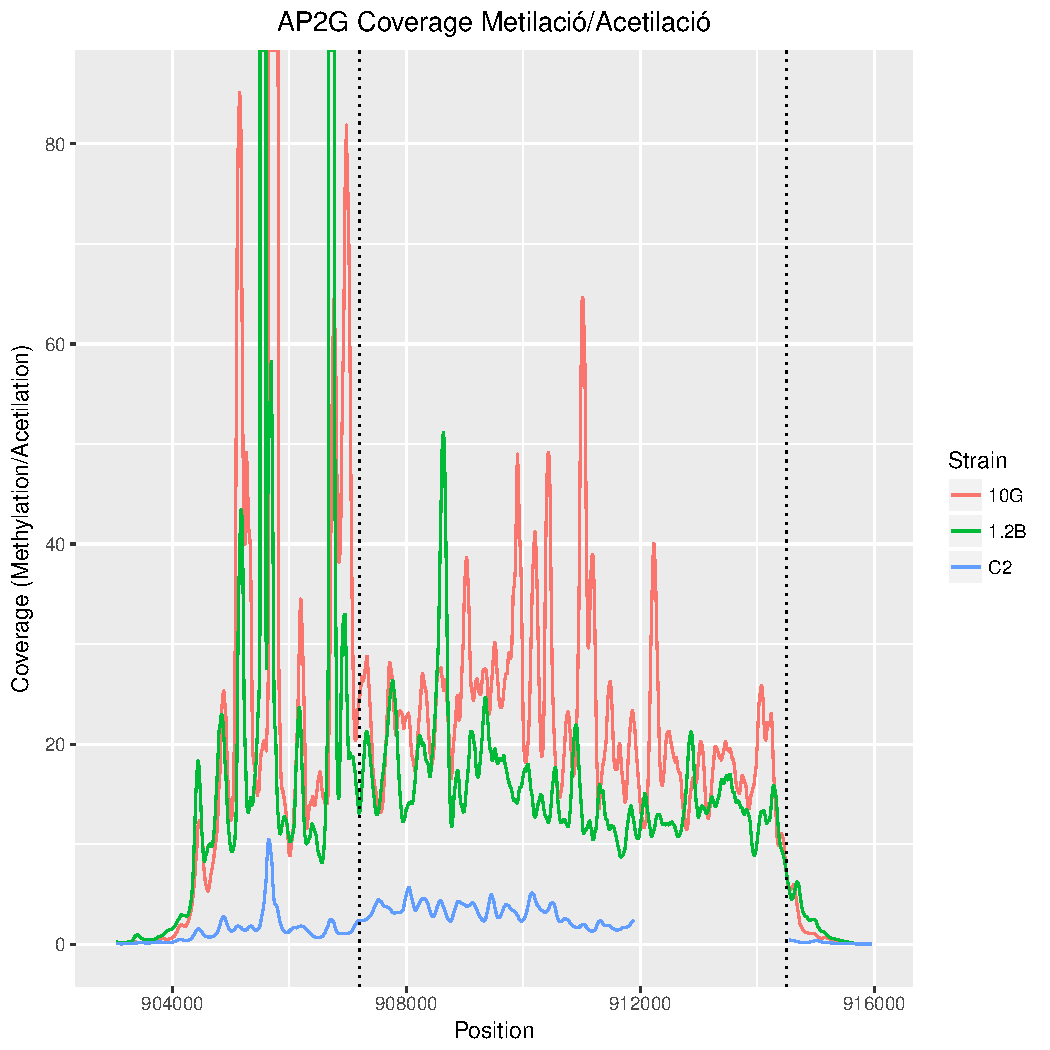
\includegraphics[width=1\linewidth]{figure/Met_Ac-1} 

\end{knitrout}
\end{document}
